\section{Руководство по установке\\ и использованию приложения}
\label{sec:inst}

Для корректной работы клиентского приложения необходим мобильный телефон следующей минимальной конфигурации:

\begin{itemize}
  \item ОС: Android версии не ниже 4.5 или iOS не ниже 7 версии с предустановленным браузером;
  \item карта памяти на мобильном устройстве: 20Мб свободного места;
  \item ОЗУ: 523 Мб;
  \item процессор: Exynos 5410 или аналогичный Snapdragon или Apple A7 и выше.
\end{itemize}

Для запуска клиентского приложения необходимо установить приложение на мобильное устройство. Для этого необходимо иметь скомпилированную версию приложения с разрешениями: apk для Android устройств или ipa для устройств iOS. После чего необходимо установить приложение на мобильное устройство. 

Для запуска необходимо на мобильном устройстве найти приложение FH и запустить его, это позволит увидеть стартовую страницу приложения, показанную на рисунке~\ref{fig:inst:page:login}.

\begin{figure}[ht]
\centering
  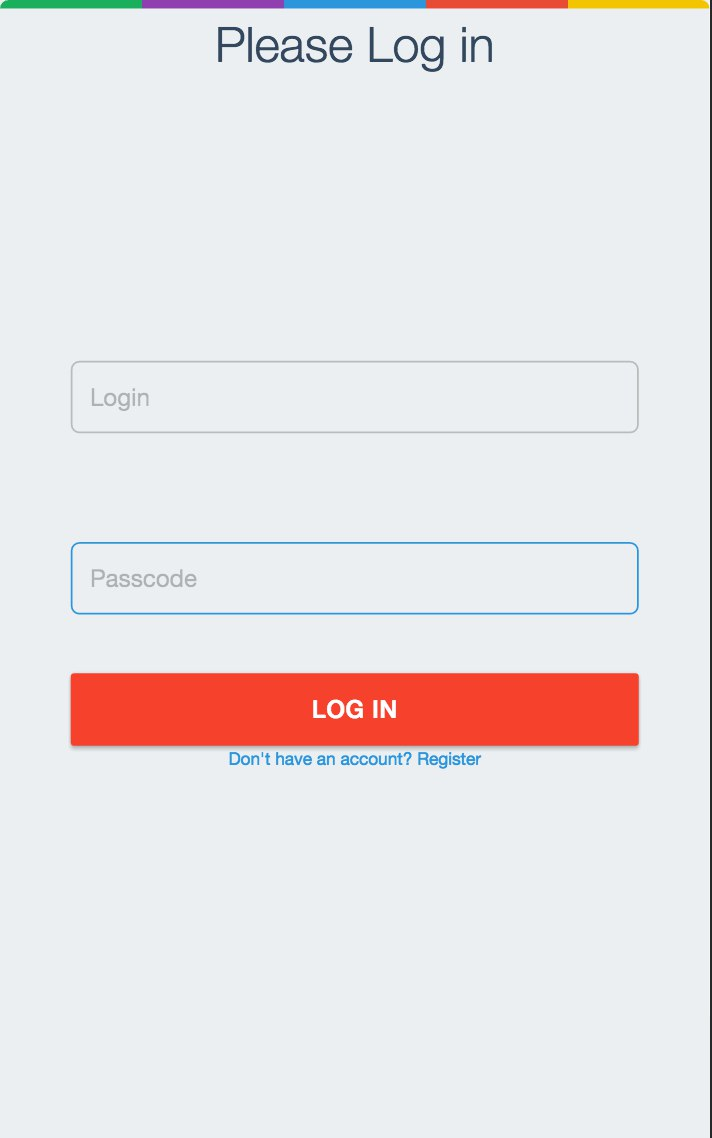
\includegraphics[scale=0.2]{loginPage.jpg}  
  \caption{Стартовая страница}
  \label{fig:inst:page:login}
\end{figure}

Для входа в систему необходимо иметь учетную запись, если учетной записи не существует, то ее можно создать используя ссылку <<Don't have account>>.

После того, как пользователь залогинился, он попадает на страницу с выбором действия, показанную на рисунке~\ref{fig:inst:page:main}, которое он собирается произвести. Приложение позволяет произвести несколько действий:
\begin{itemize}
  \item посмотреть все виды медицинских заключений за все время;
  \item произвести импорт с изображения, которое уже есть на карте памяти;
  \item сделать новую фотографию и произвести импорт;
  \item конвертировать все виды карточек в PDF-документ.
\end{itemize}

Также в шапке самой страницы есть имя пользователя приложения, а также кнопка настроек, которая позволит пользователю либо выйти из приложения, либо изменить некоторые данные о себе.

\begin{figure}[ht]
\centering
  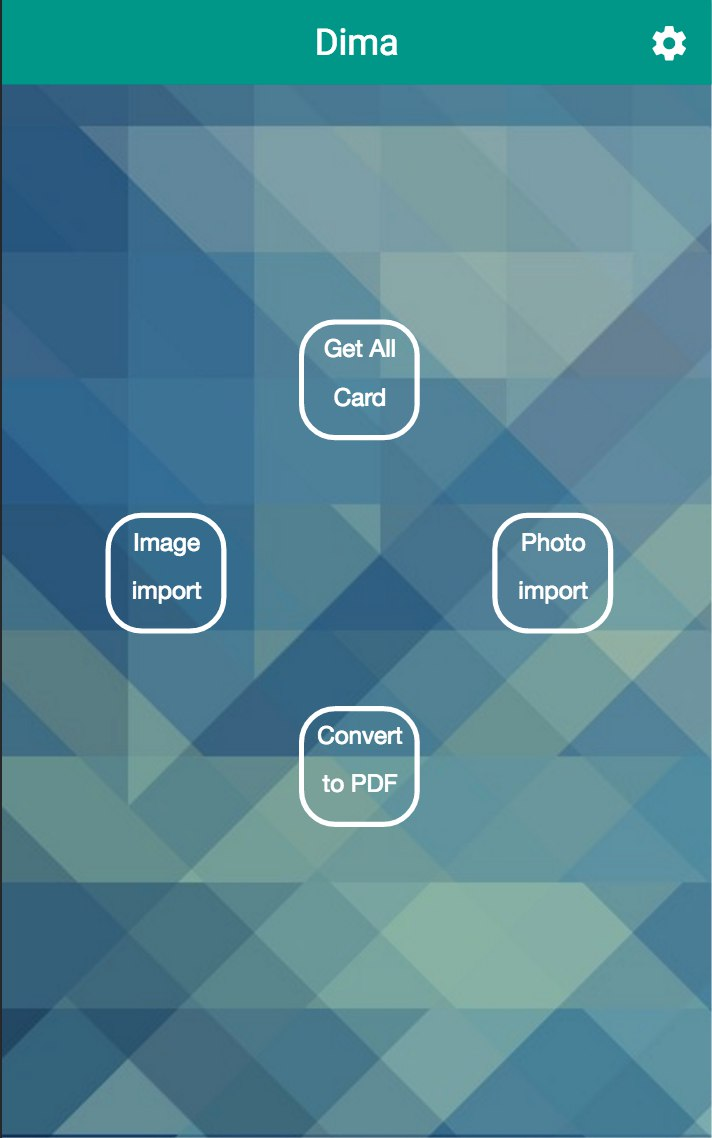
\includegraphics[scale=0.2]{mainPage.jpg}  
  \caption{Содержание главной страницы приложения}
  \label{fig:inst:page:main}
\end{figure}

Чтобы произвести манипуляцию с медицинскими заключеними, необходимо нажать на кнопку <<Get All Card>>, которая перенаправит вас на страницу списка карточек, которая показана на рисунке~\ref{fig:inst:page:listMedical}. 

На этой странице можно либо добавить новое медицинское заключение, полученное в медицинском центре, либо посмотреть текущие заключения. Для добавления нового медицинского заключения необходимо нажать на кнопку <<+>>, а для перехода на уже существующее заключение, необходимо просто выбрать из списка нужное заключение и нажать на него.

\begin{figure}[ht]
\centering
  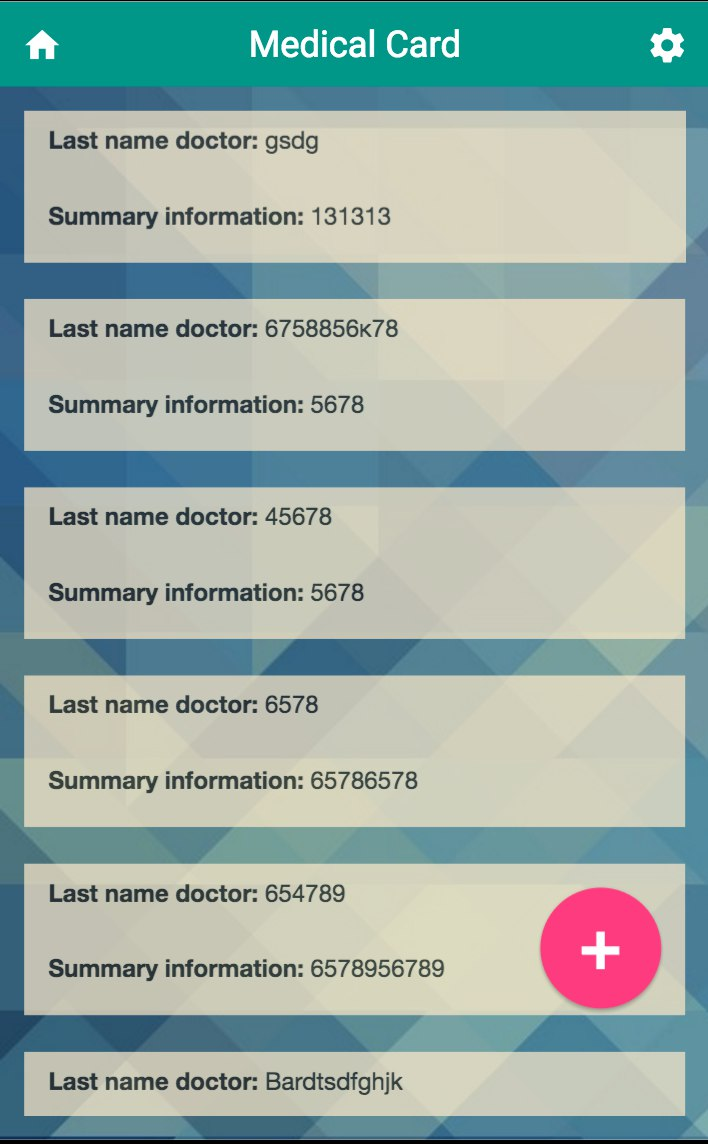
\includegraphics[scale=0.2]{listMedicalPage.jpg}  
  \caption{Содержание страницы списка медицинских заключений}
  \label{fig:inst:page:listMedical}
\end{figure}

Для импорта фотографии, необходимо нажать на главной странице кнопку <<Photo Import>> или <<Image Import>> в зависимости от того, есть ли необходимость делать новую фотографию. Если такой необходимости нету, то будет предложен список приложений на мобильном устройстве, которые позволяют открывать фотографии устройства. Из этих фотографий, необходимо будет выбрать фотографию медицинского заключения и передать приложению.

Если необходимость в новой фотографии есть, то приложение после нажатия на кнопку <<Photo Import>> откроет вам камеру устройства, при помощи которой можно произвести снимок медицинского заключения и в последствии передать приложению на обработку.

\begin{figure}[ht]
\centering
  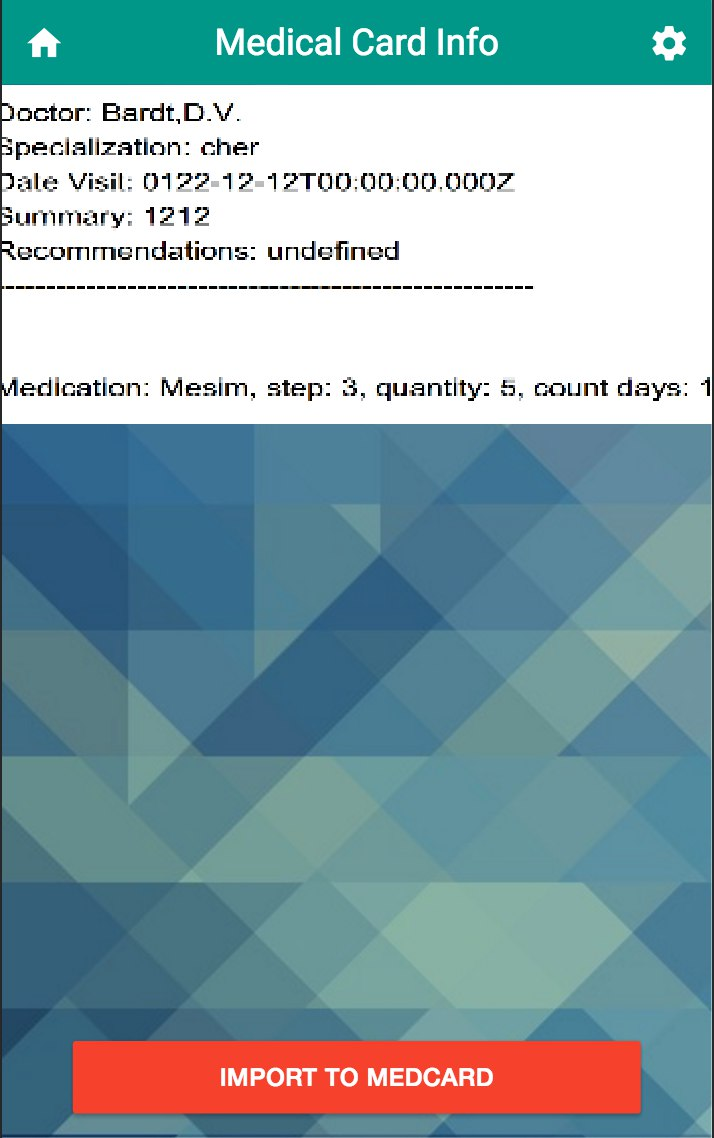
\includegraphics[scale=0.55]{importPage.jpg}  
  \caption{Содержание страницы обработки фотографии медицинского заключения}
  \label{fig:inst:page:importMedical}
\end{figure}

Страница обработки фотографии выглядит как на рисунке~\ref{fig:inst:page:importMedical}. Чтобы запустить обработку и анализ, полученной фотографии, необходимо нажать на кнопку <<Import To Medcard>>, после которой начнется анализ фотографии и запустится спиннер, который даст пользователю понять, что приложение занимается обработкой изображения.